\chapter{Oscilloscope: High level implementation}
    The following chapter gives insights on the high level implementation of $\Delta$QSD in the oscilloscope.
    \begin{itemize}
        \item We first provideinsights into how $\Delta$QSD was implemented in the oscilloscope, the parameters that define a probe's $\Delta$Q, its representation and what can be done with $\Delta$Qs. We show how a probe $\Delta$Q will be shown in the oscilloscope
        \item We then provide a language to write outcome diagrams based on an already existing syntax.
        \item Lastly, we explain how to control the system in the oscilloscope and how to interact with the stub
    \end{itemize}

\section{$\Delta$Q implementation}

Originally, $\Delta$Q(x) denotes the probability that an outcome occurs in a time $t \le x$, defining then the "intangible mass" of such IRV as $1 - \lim_{x\to\infty} \Delta Q (x)$.
We then extend the original definition to fit real time constraints, needing to calculate $\Delta$Qs continuously.

For a given observable, $\Delta$Q($t_l$, $t_u$, $dMax$) is the probability that the time of series with samples between time $t_l < t_u$, an observable occurs in time t $\le$ dMax.


\subsection{Internal representation of a $\Delta$Q}
    We provide a $\Delta$Q class to calculate the $\Delta$Q of an observable between a lower time bound $t_l$ and an upper time bound $t_u$.
    The $\Delta$Q can be calculated in various ways: \\
    The first way is by having $n$ collected samples between $t_l$ and $t_u$ and calculating its PDF and then calculating the \textit{empirical cumulative distribution function} (ECDF) based on its PDF.
    A $\Delta$Q can also be calculated by performing operations on two or more $\Delta$Qs, the notion of samples is then lost between calculations, as the interest shifts towards the calculate PDFs and ECDFs.
    Below, is how both are calculated given $n$ samples.
    \subsubsection{PDF}
  We approximate the PDF of the observed random variable $\textbf{X}$ via a histogram. We partition the values into $N$ bins of equal width, this is required to ease future calculations.
        Given $\lbrack x_i, x_{i+1} \rbrack$ the interval of a bin $i$, where $x_i = i\Delta x$, and $\hat{p}(x_i)$ the value of the PDF at bin $i$, for $n$ bins:
        \begin{equation}
            \begin{cases}
                \hat{p}(i) = \dfrac{n_i}{n}, \text{if } i \le n \\
                \hat{p}(i) = \hat{p}(n), \text{if } i > n \\
            \end{cases}
            \label{eq:pdf}
        \end{equation}
   With $n_i$ the number of successful samples whose elapsed time is contained in the bin $i$, $n$ the total number of samples.
    \subsubsection{ECDF}
    The value $\hat{f}(x_i)$ of the ECDF at bin $i$ with $n$ bins can be calculated as:
    \begin{equation}
        \begin{cases}
            \hat{f}(i) = \sum_{j=1}^{i} \hat{p}(j), & \text{if } i \le n \\  
            \hat{f}(i) = \hat{f}(x_n), & \text{if } i > n 
        \end{cases}
        \label{eq:cdf}
    \end{equation}
    
    \subsection{dMax}
        The key concept of $\Delta$QSD is having a maximum delay after which we consider that the execution is failed, this is represented in an observable as $dMax$. The user defines, for each observable the maximum delay its execution can have. \\ 
Setting a maximum delay for an observable is not a job that can be done one-off and blindly, it is something that is done with an underlying knowledge of the system inner-workings and must be thoroughly fine tuned during the execution of the system by observing the resulting distributions of the obtained $\Delta$Qs. \\

We define in our oscilloscope a formula to dynamically define a maximum delay based on the formula:
\begin{equation}
    dMax = \Delta_{t base} * 2^n * N  
    \label{eq:dMax}
\end{equation}
Where:
\begin{itemize}
    \item $\Delta_{t base}$ represents the base width of a bin, equal to 1ms.
    \item $N$ the number of bins.
\end{itemize}

Some tradeoffs must though be acknowledged when setting these parameters, a higher number of bins corresponds to a higher number of calculations and space complexity, a lower $dMax$ may correspond to more failures. These are all tradeoffs that must be considered by the system engineer and set accordingly.
    \begin{figure}[H]
        \begin{center}
            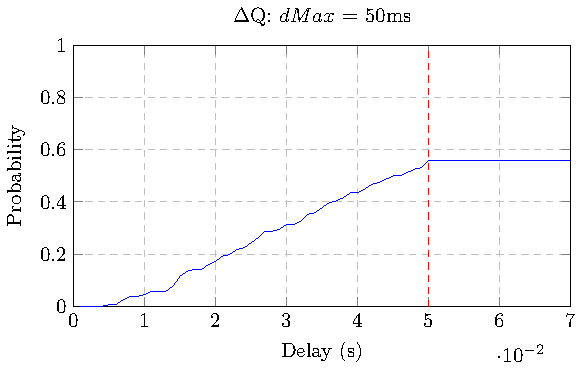
\includegraphics[width=\textwidth, scale = 0.6]{tikz/cdf_dmax.pdf}
        \end{center}
        \caption{$\Delta$Q: $dMax$ = 50ms, the CDF will stay constant when delay $> dMax$}
    \end{figure}

    \subsection{QTA}
        A simplified QTA is defined for observables. We define 4 points for the step function at 25, 50, 75 percentile and the maximum amount of failures accepted for an observable. An observed $\Delta$Q will calculate that based on the samples collected. 
\subsection{Operations}
    In a previous section [REF HERE] we talked about the possible operations that can be performed on and between $\Delta$Qs, the time complexity of FTF, ATF and PC is trivially $\mathcal{O}(N)$ where N is the number of bins. As to convolution, the naïve way of calculating convolution has a time complexity of $\mathcal{O}(N^2)$, this quickly becomes a problem as soon as the user wants to have a more fine-grained understanding of a component. Below we present two ways to perform convolution.

        \subsubsection{Convolution}
        
        \paragraph{Naïve convolution}
        Given two $\Delta$Q binned PDFs $f$ and $g$, the result of the convolution $f \circledast g$ is given by 
        \begin{equation}
            (f \circledast g)\lbrack n \rbrack = \sum_{m = 0}^{N} = f\lbrack m \rbrack g \lbrack n - m \rbrack  
            \label{eq:discconv}
        \end{equation}
            

    \paragraph{Fast Fourier Transform Convolution}
        FFTW (Fastest Fourier Transform in the West) is a C subroutine library [cite site] for computing the discrete Fourier Transform in one or more dimensions, of arbitrary input size, and of both real and complex data. We use FFTW in our program to compute the convolution of $\Delta$Qs.
    Whilst the previous algorithm is far too slow to handle a high number of bins, convolution leveraging Fast Fourier Transform (FFT) allows us to reduce the amount of calculations to $\mathcal{O}(n \text{log} n)$. \\
    FFT and naïve convolution produce the same results in our program barring $\varepsilon$ differences (around $10^{-18}$) in bins whose result should be 0.

    \subsubsection{Arithmetical operations}
        We can apply a set of arithmetical operations between $\Delta$Qs ECDFs, and on a $\Delta$Q.
    \paragraph{Scaling (multiplication)} A $\Delta$Q can be scaled w.r.t a constant $0 \le j \le 1$. It is equal to binwise multiplication on ECDF bins.
    \begin{equation}
        \hat{f_r}(i) = \hat{f}(i) \cdot j
        \label{eq:mul_ecdf}
    \end{equation}

    \paragraph{Operations between $\Delta$Qs} 
        Addition, subtraction and multiplication can be done between two $\Delta$Q of equal bin width (but not forcibly of equal length) by calculating the operation between the two ECDFs of the $\Delta$Qs:
        \begin{equation}
            \Delta \text{Q}_{AB}(i) = \hat{f_A}(i) [\cdot, +, -] \hat{f_B}(i)
            \label{eq:op_dq}
        \end{equation}
    \subsection{Confidence bounds}
    To observe the stationarity of a system we must observe a window of $\Delta$Qs of an observable and calculate confidence bounds over said windows. We present here the formulae required to give such bounds with 95\% confidence level. \\
        For a bin $i$, its mean over a window is:
            \begin{equation}
                \mu_i = \dfrac{1}{n_i} \sum_{j=1}^{n_i} x_{ij}
                \label{eq:mean_ecdf}
            \end{equation}
        Where $x_{ij}$ is a bin's $i$ value for an ECDF $j$.
        Its variance:
            \begin{equation}
                \sigma^2_i = \dfrac{1}{n_i} \sum_{j=1}^{n_i} x^2_{ij} - \mu^2_i
                \label{eq:var_ecdf}
            \end{equation}
        The confidence intervals $CI_i$ for a bin $i$ can then be calculated as:
        \begin{equation}
            CI_i = \mu_i \pm z_{\alpha/2} \cdot \dfrac{\sigma_i}{\sqrt{n_i}}      
            \label{eq:ci_i}
        \end{equation}
    The bounds can be updated dynamically by inserting or removing a $\Delta$Q, this allows us to consider a small window of execution rather than observing the whole execution.

    \subsection{Rebinning}
        Rebinning refers to the aggregation of multiple bins of a bin width $i$ to another bin width $j$. \\  
        Operations between $\Delta$Qs can be done on $\Delta$Qs that have the same bin width, this is why it is fundamental that all observables have a common $\Delta_{tbase}$. This allows for fast rebinning to a common bin width. \\
        Given two $\Delta$Qs $\Delta$Q$_i$, $\Delta$Q$_j$:
        \begin{center}
            $\Delta_{Tij}$ = max \{$\Delta_{Ti}, \Delta_{Tj} \}$
        \end{center}
        and the PDF of the rebinned $\Delta$Q at bin $b$, from the original PDF of $n$ bins, where $k$ = $\frac{\Delta{_Ti}}{\Delta_{Tj}}$:
        \begin{equation}
            p'_b = \sum_{n=b \cdot k}^{b+ 1 \cdot k - 1} p_n, \quad b=0,1,\dots \lceil \frac{N}{k} \rceil  
        \end{equation}
        We perform rebinning to a higher bin width for a simple reason, while this leads to loss of information for the bin with the lowest bin width, rebinning to a lower bin width would imply inventing new values for the $\Delta$Q with the highest bin width.
       
        
        \begin{figure}[H]
            \begin{center}
                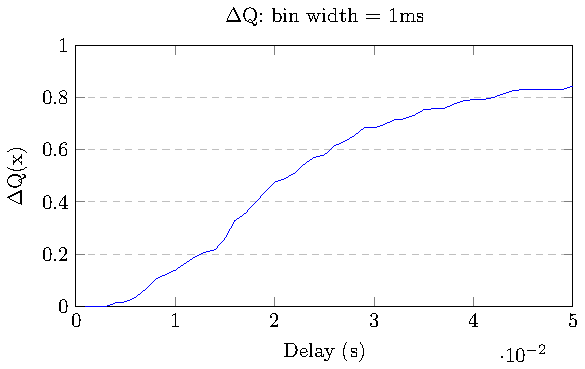
\includegraphics[width=\textwidth]{tikz/cdf.pdf}
            \end{center}
            \caption{Sample $\Delta$Q with 1ms bins}
        \end{figure}

 
        \begin{figure}[H]
            \begin{center}
                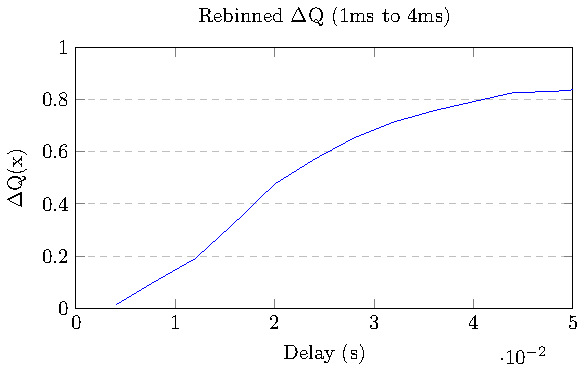
\includegraphics[width=\textwidth]{tikz/rebinned_cdf.pdf}
            \end{center}
            \caption{Previous $\Delta$Q after rebinning to 4ms bins}
        \end{figure}

\section{$\Delta$Q display}
    An observable's displayed graph must contain the following functions:
    \begin{itemize}
        \item The mean and confidence bounds of a window of previous $\Delta$Qs
        \item The observed $\Delta$Q($t_l, t_u, dMax$)
        \item For a probe, the calculated $\Delta$Q from its components.
        \item Its QTA
    \end{itemize}
    This allows for the user to observe if a $\Delta$Q has deviated from normal execution, analyse its stationarity, nonlinearity and observe its execution.
    \begin{figure}[!ht]    
    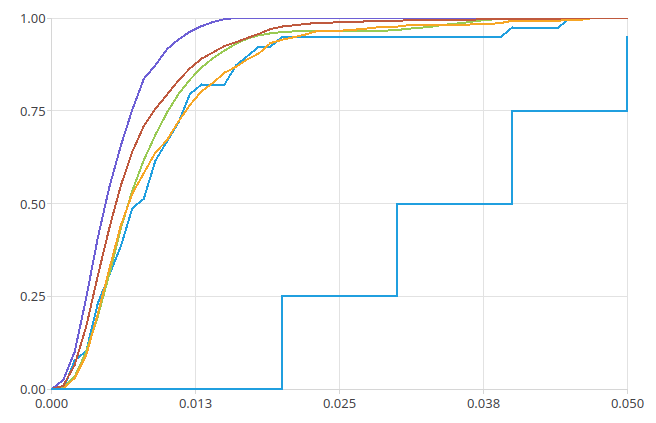
\includegraphics[scale =0.8, width=\textwidth]{img/dqdispl.png}
    \end{figure}

  \section{Outcome diagram}
        An abstract syntax for outcome expressions and consequently outcome diagrams has already been defined in a previous paper \cite{art}, nevertheless, the oscilloscope provides additional features not included in the original syntax and, moreover, needs a textual way to define an outcome diagram. 
       
        We define thus a grammar to create an outcome diagram in our oscilloscope, our grammar is a textual interpretation of the abstract syntax.
        \subsection{Probes}
            To attach probes in the oscilloscope, the user must define outcomes and probes that observe outcome expressions.
            \subsubsection{Outcome}
                In our system an outcome is defined with its name
                \begin{minted}{text}
                    ... = outcomeName;
                \end{minted}
        
        \subsubsection{Probes containing outcome expressions}
            A probe can contain one component or a sequence of causally linked components.
            The user can define as many probes that contain outcome expressions as they want, they have to be declared as follows:
            \begin{minted}{text}
                probe = component [-> component2];
                probe2 = newComponent -> anotherComponent;
            \end{minted}
    
            These probes can be reused in other probes or in the system by adding \texttt{"s:"} (subsystem) before they are used.
            \begin{minted}{text}
                probe3 = s:probe -> s:probe2;
            \end{minted}
 
        \subsection{Operators, outcome expressions}
            To build a system, we must define the relations between outcomes and outcome expressions, below is how they can be defined. 

            First-to-finish, all-to-finish and probabilistic choice must contain at least two components, this is because the operations to calculate the \textit{calculated} $\Delta$Q rely on using the CDF of the components that define the operator.
            
        \subsubsection{Causal link}
            A causal link between two components can be defined by a right arrow from \texttt{component\_i} to \texttt{component\_j}
        \begin{minted}{text}
            component_i -> component_j 
        \end{minted}
        
        \subsubsection{All-to-finish operator}
            An all-to-finish operator needs to be defined as follows:
            \begin{minted}{text}
                a:name(component1, component2...)
            \end{minted}

        \subsubsection{First-to-finish operator}
            A first-to-finish operator needs to be defined as follows.
            \begin{minted}{text}
                f:name(component1, component2...)
            \end{minted} 

        \subsubsection{Probabilistic choice operator}
            A probabilistic choice operator needs to be defined as follows:
            \begin{minted}{text}
                p:name[probability_1, probability_2, ... probability_i](component_1, component_2, ..., component_i) 
            \end{minted}
            In addition to being comma separated, the number of probabilities inside the brackets must match the number of components inside the parentheses. For $n$ probabilites $p_i$, $0 < p_i < 1$, $\sum_{i = 0}^{n} p_i = 1$ 
        
            
        \subsection{Limitations}
            Our system has a few limitations compared to the theoretical applications of $\Delta$Q, namely, no cycles are allowed in the definition of a system.
        
        \begin{minted}{text}
            probe = s:probe_2;
            probe_2 = s:probe;
        \end{minted}
        The above example is not allowed and will raise an error when defined.  



\section{Dashboard}
    The dashboard is devised of multiple sections where the user can interact with the oscilloscope, create the system, observe the behaviour of its components, set triggers.

    \subsection{Sidebar}
        The sidebar has multiple tabs, we explain here the responsibility of each one.

    \subsubsection{System/Handle plots tab}

    \paragraph{System creation}
        In this tab the user can create its system using the grammar defined before, he can save the text he used to define the system or load it, the system is saved to a file with any extension, we nevertheless define an extension to save the system to, the extension \texttt{.dq}.
        If the definition of the input is wrong, he will be warned with a pop up giving the error the parser generator encountered in the creation of a system.

    \paragraph{Adding a plot}
        Once the system is defined, the user can choose the probes he wants to plot. They can select multiple probes per plot and display multiple plots on the oscilloscope window.
    
    \paragraph{Polling rate}
        The user can choose the polling rate of the system: How often $\Delta$Qs are calculated and displayed in the oscilloscope.

    \paragraph{Editing a plot}
        By clicking onto a plot that is being shown, the user can choose to add or remove probes to and from it. Multiple probes can be selected to either be removed or added.

    \subsubsection{Parameters tab}
        In this tab, the user can define parameters for the probes they have defined.

    \paragraph{Set a QTA}
        The user is given the choice to set a QTA for a given observable, they have 4 fields where they can fill in which correspond to the percentiles and the maximum amount of failures allowed, they can change this dynamically during execution.

    \paragraph{dMax, bins}
        The user has a slider which goes from -10 to 10, where they can set the parameters we explained previously, $n$, the exponent of $\Delta_{tbase} \cdot 2^n$ and the bins $N$. When these informations are saved by the user, the new $dMax$ is transmitted to the stub and saved for the selected observable.

    \subsubsection{Triggers tab}
        In the triggers tab the user can set triggers and observe the snapshots of the system.

    \paragraph{Set triggers}
        The user can set which triggers to fire for the probes they desire, they are given checkboxes to decide which ones to set as active or not (by default, the triggers are deactivated).
    
    \paragraph{Fired triggers}
        Once a trigger is fired, the system start a timer, during which all probes start recording the observed $\Delta$Qs (and the calculated ones if applicable) without discarding older ones. Once the timer expires, the snapshot is saved for the user in the triggers tab. In the dashboard, it indicates when the trigger was fired (timestamp) and the name of the probe which fired it.
    
    \subsection{Plots window}
        To the left, the main window shows the plots of the probes being updated in real time. 

    \subsection{Stub controls}
        Below the sidebar, two buttons are present, these buttons communicate to the stub. 
         
        The \textbf{start stub} button sends a message to the stub, telling it to start sending spans. The \textbf{stop stub} button stops it.

%\section{Triggers}
    Like an oscilloscope that has a trigger mechanism that fires when a signal of interest is recognized by the oscilloscope, our $\Delta$Q oscilloscope has a similar mechanism of triggers that are fired when an observed $\Delta$Q violates certain conditions. Let us define what these triggers are.

    \subsection{Load}
        A trigger on an observed $\Delta$Q can be fired if 
    \begin{center}
        nSamples($\Delta$Q($t_l, t_u, dMax$)) > maxAllowedSamples 
    \end{center}

    \subsection{QTA}
        There are two possible [can change] triggers that can be fired based on the observable defined $\Delta$Q's QTA.   
        \subsubsection{Percentiles}
            A trigger can be fired if:
        \begin{center}
            $\Delta$Q$_{obs}$[percentile] $<$ observableQTA$_{req}$[percentile] \quad $\forall \text{ percentile } \{0.25, 0.5, 0.72\}$
        \end{center}
        \subsubsection{Failure}
            A trigger can be fired on the percentage of failed samples for $\Delta$Q($t_l, t_u, dMax$) if:
        \begin{center}
            success($\Delta$Q$_{obs}$) $<$ success(observableQTA$_{req}$)
        \end{center}

    \subsection{Time series snapshots}
        When a trigger is fired, the oscilloscope will capture ...


